\section{Zaključak}

Razvijena aplikacija omogućava jednostavno upravljanje osnovnim režimima rada
AD9850 integrisanog kola. \\
RPi se pokazao kao dobra platforma za razvoj korisničkog interfejsa generatora
funkcija i ostavlja mogućnost za lako proširenje funkcionalnosti. \\

\subsubsection{Predlozi proširenja}
U nastavku biće predloženi načini za proširenje ovog projekta.
Implementacijom ovih predloga može se dobiti uređaj za testiranje uređaja u oblasti audio elektronike
i drugih oblasti na višim frekvencijama. \\
Većina ovih predloga zahteva projektovanje dodatnih analognih
elektronskih kola pa zbog toga njihova implementacija nije razmatrana u ovom projektu. \\

\begin{itemize}
\item \textbf{Dodavanje izlaznog pojačavača} sa mogućnosti dodavanja
  offset napona kako bi se obezbedili standardni naponski nivoi prisutni kod
  komercijalnih generatora funkcija (+,- 15V). \\
  Zbog relativno širokog opsega frekvencija generisanog signala (0-40MHz) ovo
  nije trivijalan zadatak i potrebno je korišćenje odgovarajućeg operacionog
  pojačavača sa dovoljno širokim frekventnim opsegom, alternativno ograničiti
  izlaznu frekvenciju na uži opseg.

\item \textbf{Softversko podešavanje ispune pravougaonog signala}. \\
  Modul korišćen u ovom projektu nema spoljni pristup ulazu internog komparatora i
  potrebno je izvršiti modifikaciju na ploči ili projektovati novu ploču.
  Potrebno je obezbediti analogni napon sa mogućnosti podešavanja softverskim
  putem, najverovatnije korišćenjem integrisanog \textbf{AD} konvertora.

\item \textbf{Proširenje projekta na Wobbler generator}. \\
  Realizovan sweep režim rada predstavlja osnovu Wobbler generatora. \\
  AD9850 je pogodan za realizaciju ovog uređaja zbog širokog opsega izlazne
  frekvencije i mogućnosti brze promene frekvencije. \\
  Pored Sweep signala potrebno je obezbediti i trougaoni signal za vremensku
  bazu osciloskopa kao i potrebne pojačavače za oba signala.

\end{itemize}

\subsubsection{Slike rada}

U nastavku su prikazane slike sa logičkog analizatora koje prikazuju rad uređaja.
Pošto je analogni signal sniman logičkim analizatorom moguće je videti samo dva
naponska nivoa, tako da se ne može videti oblik sinusoide i njena čistoća.
Može se videti perioda sinusoide i njeno trajanje. \\

\begin{figure}[H]
  \centering{
    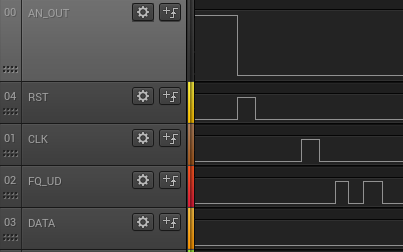
\includegraphics[width=10cm]{img/capture/rst.png}
    \caption{Reset sekvenca}
    \label{reset_seq_la}
  }
\end{figure}

\begin{figure}[H]
  \centering{
    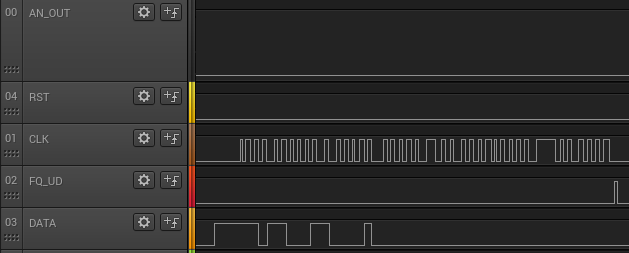
\includegraphics[width=12cm]{img/capture/data_write.png}
    \caption{Serijski upis}
    \label{serial_write_la}
  }
\end{figure}

\begin{figure}[H]
  \centering{
    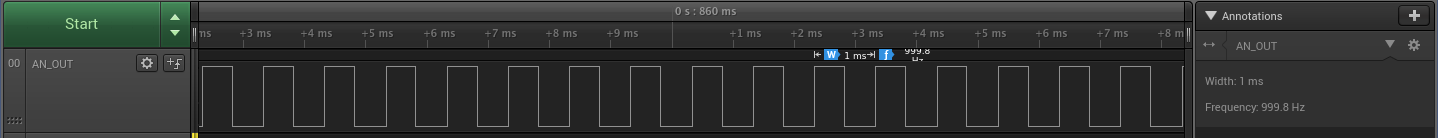
\includegraphics[width=18cm]{img/capture/an_out1khz.png}
    \caption{Run režim, frekvencija 1kHz}
    \label{run_1khz_la}
  }
\end{figure}

\begin{figure}[H]
  \centering{
    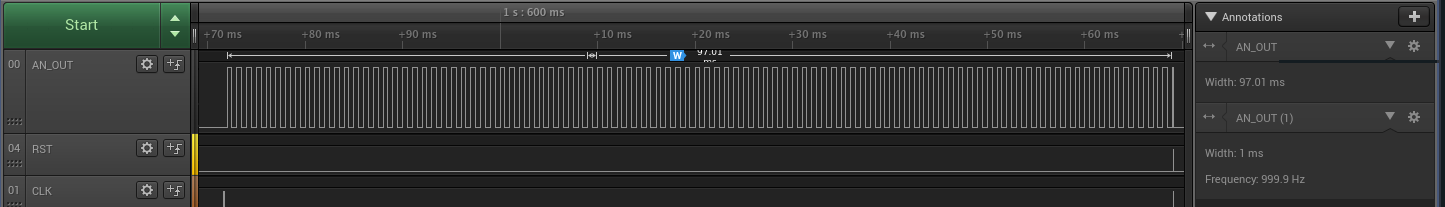
\includegraphics[width=18cm]{img/capture/run_for_100ms_1khz.png}
    \caption{Run for režim, 1kHz 100ms}
    \label{run_for_la}
  }
\end{figure}

\begin{figure}[H]
  \centering{
    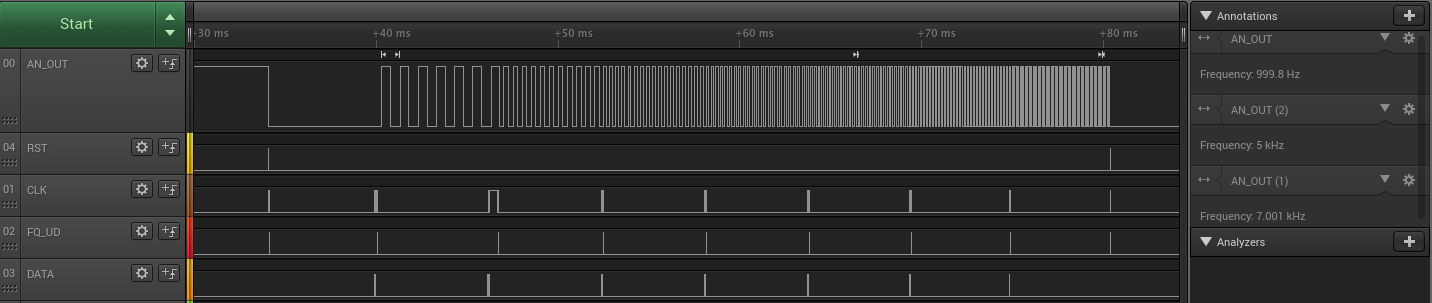
\includegraphics[width=18cm]{img/capture/sweep_1000_8000_1000_5.png}
    \caption{Sweep režim, 1kHz do 7kHz, korak od 1kHz i vreme koraka 50ms}
    \label{sweep_la}
  }
\end{figure}